\label{sec:losning}
\subsection{Dataflyt fra bilen til brukergrensesnitt}
Hele løsningen rundt å få data fra bilens telemetrimodul til brukergrensesnittet er realisert med noen enkle modulerer som gjør hver sin jobb for å frakte dataene. Dataflyten mellom de forskjellige modulene er visualisert i \ref{fig:dataflow}.

\begin{figure}[H]
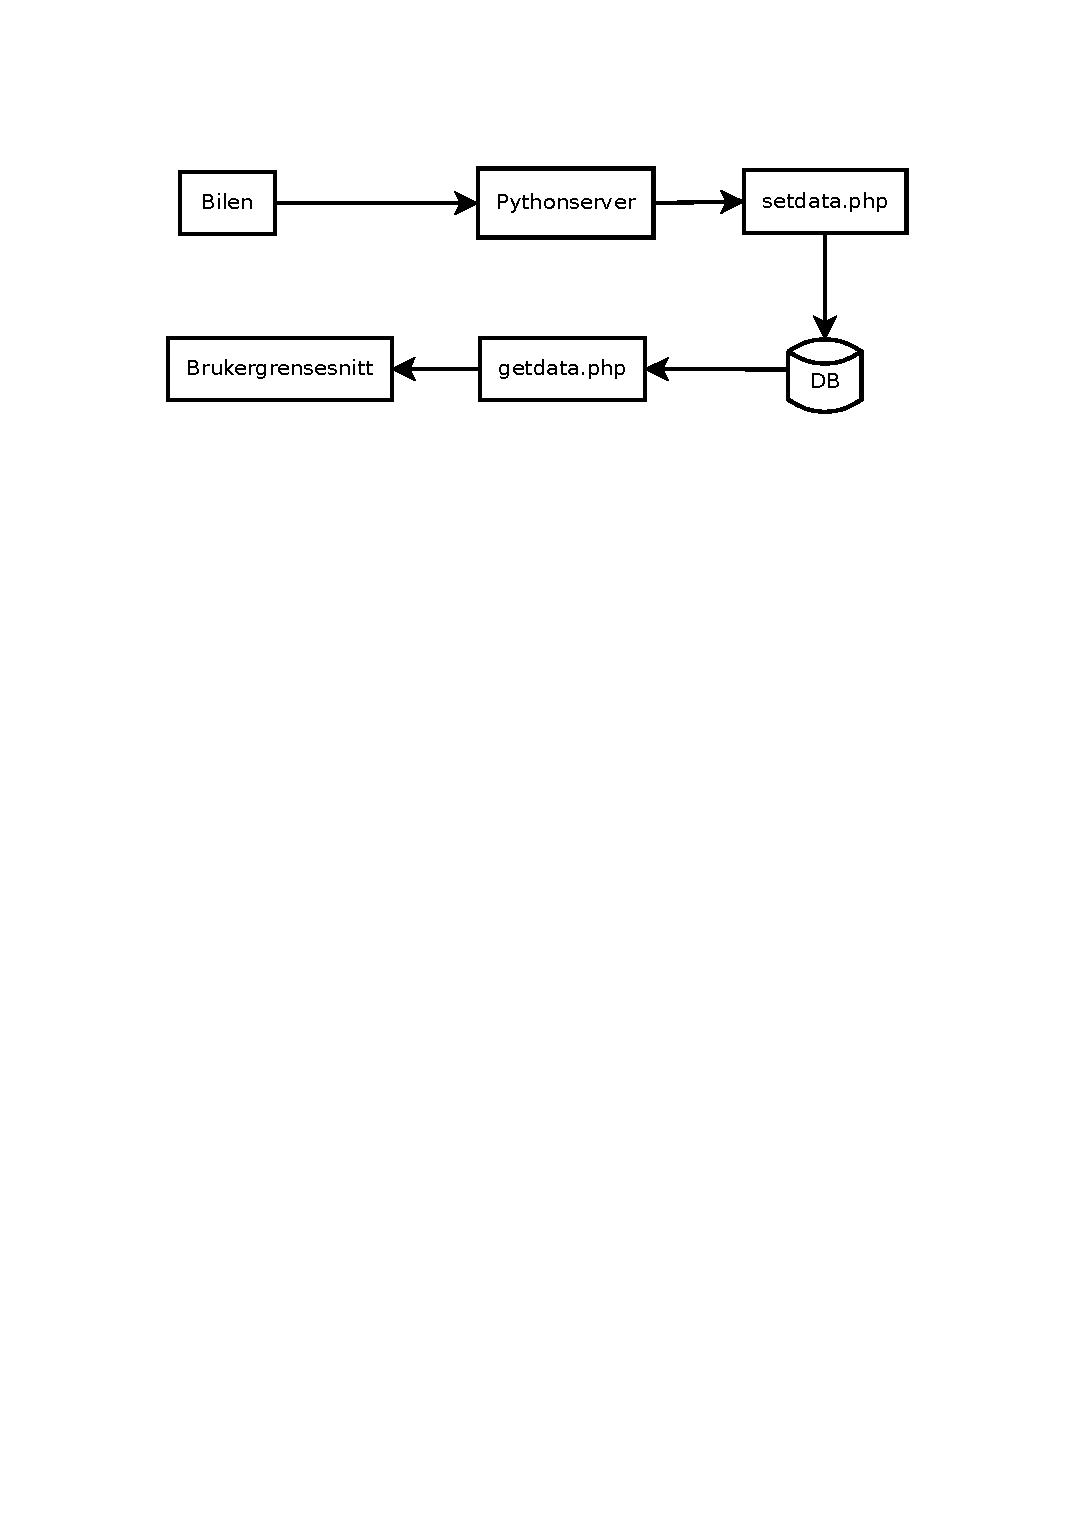
\includegraphics[width=\textwidth, trim=0 540 0 75]{images/dataflow.pdf}
\caption{Dataflyt}
\label{fig:dataflow}
\end{figure}

\paragraph{Databasen}
Databasen som kjører bak alt er en enkel MySQL-database, denne holder historikk på sensorer, tider og andre data som må være persistente. Et ER diagram over databasen kan sees i \ref{fig:er}. Tabellen config er egentlig bare en enkelt rad rad fordi den skal holde globale variable for hvorvidt løpet er startet og hvor de andre dataene kan hentes fra.

\begin{figure}[H]
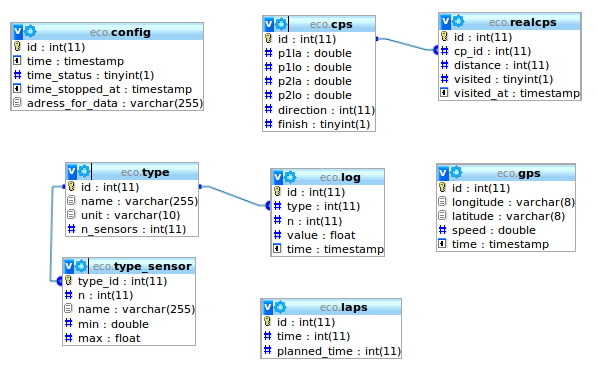
\includegraphics[width=\textwidth]{images/er.png}
\caption{Databasen}
\label{fig:er}
\end{figure}

\paragraph{Pythonserver}
Pythonserver er et lite script skrevet i Python som setter opp en TCP socket for å motta data som telemetrimodulen sender. Så fort den har mottatt en hel pakke med data fra bilens telemetrimodul gjør den en omregning av gpsposisjonene fra grader og minutter til rene grader på decimalformat. Deretter sender den dette videre ved å sette opp en HTTP connection til webserveren og sender dataene som et POST request til setdata.php.
\paragraph{setdata.php}
Denne modulen tar imot kommaseparerte data fra Pythonserveren og setter disse inn i databasen. I tillegg gjør den utregninger i forhold til om bilen har passert kontrollpunkt og oppdaterer tidstabellen i henhold til dette hvis løpet er startet fra brukergrensesnittet.
\paragraph{getdata.php}
Denne brukes for å hente data fra databasen når websiden vises. Den slår opp i databasen og bygger opp et script med jQuery\cite{jquery} som igjen oppdaterer elementer i guiet.
\subsection{Brukergrensesnitt}
Brukergrensesnittet er bygget uten hjelp av noe spesielt rammeverk, men i stedet bygget fra grunnen ved hjelp av PHP, javascript og jQuery\cite{jquery}. Det kjører en jqueryfunksjon som hver x. minutt henter et nytt script som getdata.php genererer og oppdaterer elementene i brukergrensesnittet med det. Brukergrensesnittet har et kart som bruker api fra google for å sette logoen til fuelfighter på kartet og få den til å bevege seg utifra data fra bilen. Hastigheten til bilen blir gjengitt ved hjelp av et speedometer fra Bindows Gauges\cite{bindows}. En oversikt over hvordan det ferdige systemet ser ut kan sees in en skjermdumpen \ref{fig:gui}. Stoppeklokken som sees på toppen her drives av et lite javascript. Ved å klikke på Start så settes et tidspunkt i databasen og klokka begynner å gå, dette tidspunktet brukes så av setdata.php for å regne ut rundetider på banen. Hvis det trykkes på Stop så stoppes klokka slik at brukeren kan stoppe løpet ved uforutsette hendelser.

\begin{figure}[H]
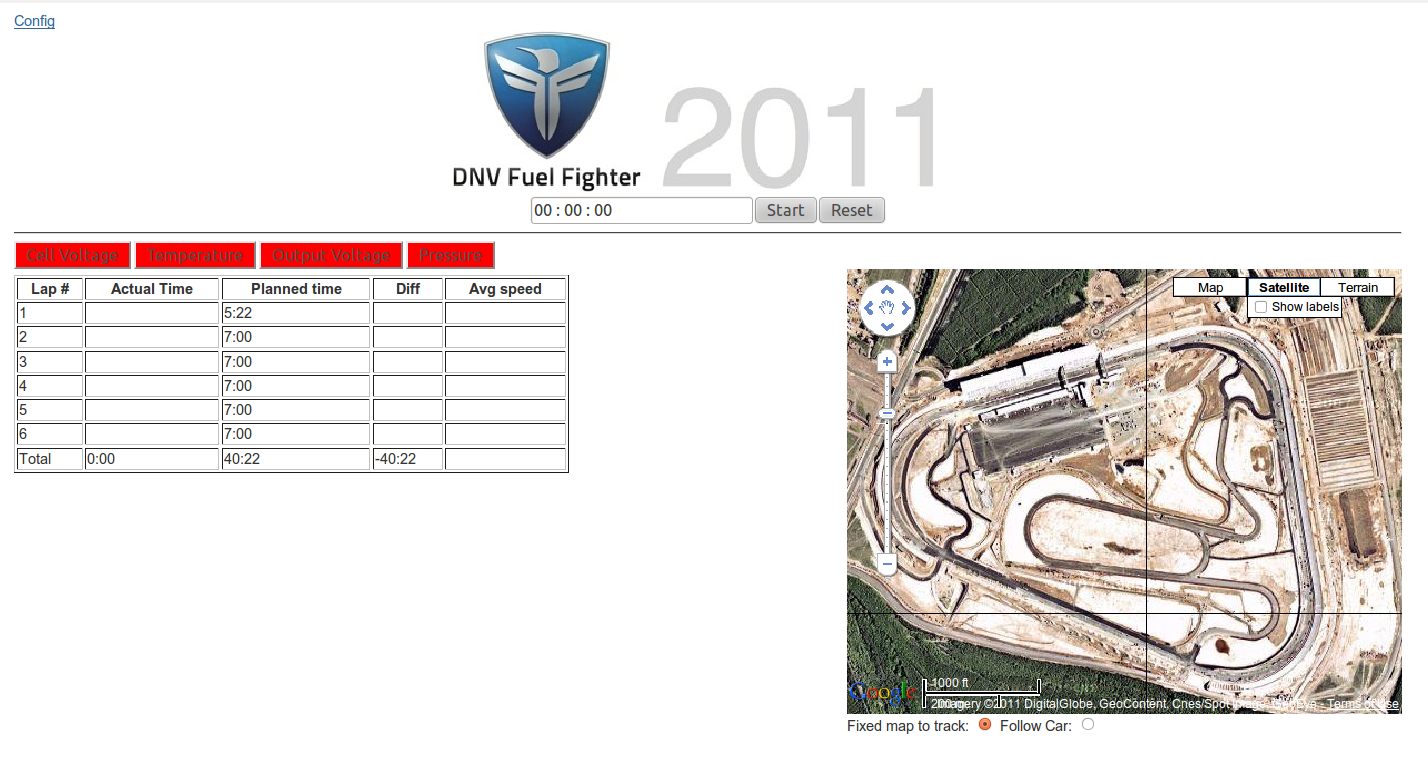
\includegraphics[width=\textwidth]{images/gui.png}
\caption{Ferdig system} 
\label{fig:gui}
\end{figure}

\paragraph{Konfigurasjon}
Det finnes også et brukergrensesnitt for at brukeren av systemet skal kunne sette navn, måleenhet og grenseverdi på sensorer. I tillegg kan også planlagte tider og hvor dataene skal hentes fra settes her.
En skjermdump av dette finnes i \ref{fig:config}, dette kommer opp som et vindu over grensesnittet i \ref{fig:gui}.

\begin{figure}[H]
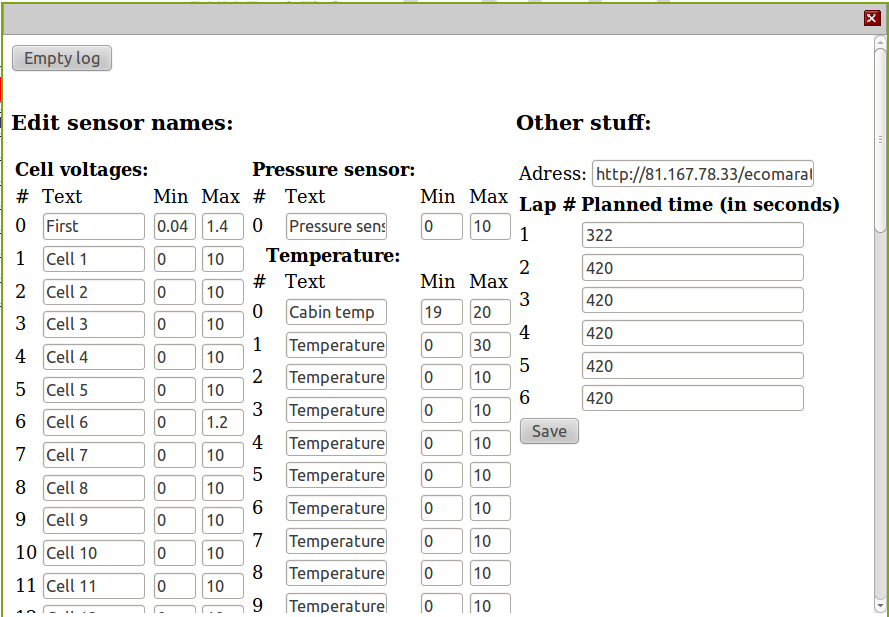
\includegraphics[width=200px]{images/config.png}
\caption{Config}
\label{fig:config}
\end{figure}

\paragraph{Statistikk}
Hver sensor kan trykkes på og da kommer vinduet som er vist i \ref{fig:stats} opp, dette genereres ut i fra det som blir lagt inn av databasen. Her kan man navigere frem og tilbake i historien for å finne ut når en sensor har meldt om feil. Grafen tegnes opp ved hjelp av biblioteket highcharts \cite{highcharts}.

\begin{figure}[H]
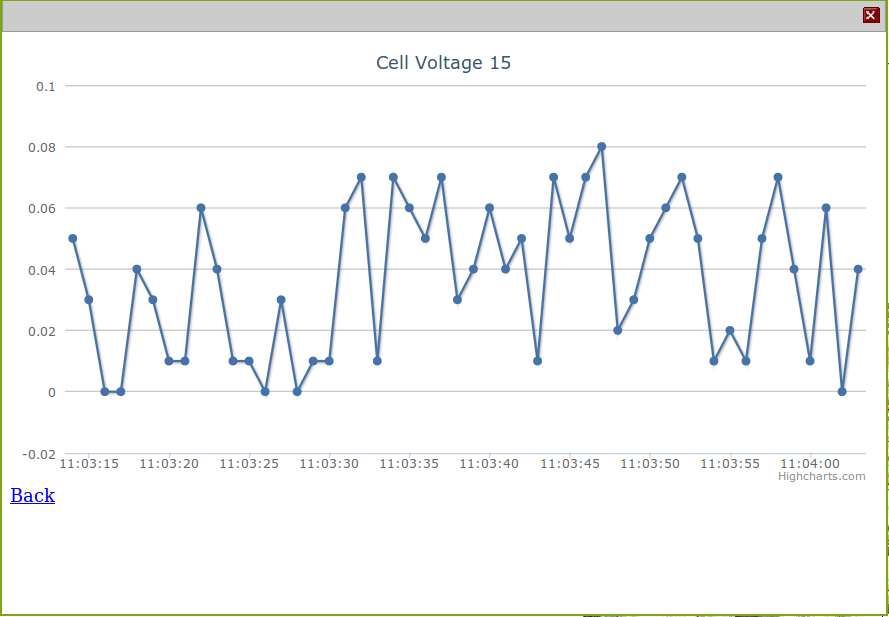
\includegraphics[width=200px]{images/stat.png}
\caption{Statistikk}
\label{fig:stats}
\end{figure}

\subsection{Telemetrimodul}
Telemetrimodulen ble laget av Anders Guldahl \cite{telemetrithesis} i 2009. Denne har ikke blitt endret mye på, men noen endringer måtte gjøres for at den skulle fungere sammen med brukergrensesnittet.
Slik det var, så leverte telemetrimodulen GPS data kun til dashbordet i bilen og hastigheten til bilen ble aldri brukt. Dette er nå endret slik at telemetrimodulen sender disse dataene sammen med de andre måleverdiene som en kommaseparert string via GPRS til Pythonserveren.
